\documentclass{beamer}

\usepackage[english]{babel}
\usepackage[utf8]{inputenc}
\usepackage{listings}
\usepackage{datetime}
\usepackage{graphics}
\usepackage{fancybox}
\usepackage{color}
\usepackage[normalem]{ulem}
\usepackage{tikz}
\usetikzlibrary{positioning}
\usepackage{hyperref}
\usetikzlibrary{shapes,arrows}
\usetheme{CambridgeUS}
\usecolortheme{seagull}
% Changing of bullet foreground color not possible if {itemize item}[ball]
\DefineNamedColor{named}{Purple}{cmyk}{0.52,0.97,0,0.55}
\setbeamertemplate{itemize item}[triangle]
\setbeamercolor{title}{fg=Purple}
\setbeamercolor{frametitle}{fg=Purple}
\setbeamercolor{itemize item}{fg=Purple}
\setbeamercolor{section number projected}{bg=Purple,fg=white}
\setbeamercolor{subsection number projected}{bg=Purple}

\renewcommand{\dateseparator}{.}
\newcommand{\todayiso}{\twodigit\day \dateseparator \twodigit\month \dateseparator \the\year}
\newcommand{\shell}[1]{\texttt{#1}}

\title{Osnove korištenja operacijskog sustava Linux}
\subtitle{01. Uvod}
\author[Antun Aleksa, Josip Žuljević]{Antun Aleksa, Josip Žuljević\\{\small Nositelj: dr. sc. Stjepan Groš}}
\institute[FER]{Sveučilište u Zagrebu \\
				Fakultet elektrotehnike i računarstva}
				
\date{\todayiso}

\begin{document}
    %\beamerdefaultoverlayspecification{<+->}
{
\setbeamertemplate{headline}[] % still there but empty
\setbeamertemplate{footline}{}

\begin{frame}
\maketitle
\end{frame}
}

\begin{frame}
\frametitle{Sadržaj}
\tableofcontents
\end{frame}

\section{Osnovni pojmovi iz operacijskih sustava}
\begin{frame}[t]
\frametitle{Operacijski sustav (1)}
\begin{itemize}
	\item Operacijski sustav ima nekoliko primarnih zadaća:
  \begin{itemize}
    \item Uspostavljanje korisničkog sučelja
    \begin{itemize}
      \item Omogućuje bezbolno izvođenje programa na bilo kojem sklopovlju
      \item Olakšava rad na računalu 'skrivanjem' raznih implementacijskih detalja
    \end{itemize}
    \item Efikasna raspodjela računalnih resursa
    \begin{itemize}
      \item Osigurava da se svaki program izvrši sigurno i neometano
    \end{itemize}
    \item Osiguravanje višeprogramskog rada
	\end{itemize}
  \item Ovakav opis je štur, ali definira najbitnije uloge
        operacijskog sustava 
\end{itemize}
\end{frame}

\begin{frame}[t]
\frametitle{Operacijski sustav (2)}
\begin{itemize}
  \item Sklopovlje – mnoštvo kompleksnih uređaja
   \begin{itemize}
     \item Pisanje aplikacija za samo jedan je komplicirano
   \end{itemize}
  \item OS preuzima detalje 
  \begin{itemize}
    \item Korisnik (u teoriji) treba znati samo što želi
    \item OS zna kako pristupiti određenom uređaju
  \end{itemize}
  \item Primjer: pisanje podataka na tvrdi disk
  \begin{itemize}
    \item Korisnik/aplikacija uputi zahtjev za brisanje datoteke
    \item OS primi zahtjev i dalje odlučuje što sa njime
  \end{itemize}
\end{itemize}
\end{frame}

\begin{frame}[t]
\frametitle{Operacijski sustav (3)}
\begin{itemize}
  \item OS je posrednik između aplikacije i sklopovlja
  \begin{itemize}
    \item korisnik $\rightarrow$ aplikacija $\rightarrow$ OS 
          $\rightarrow$ uređaj
  \end{itemize}
  \item Aplikacijama nikada nije dopušteno izravno pristupanje uređajima
  \begin{itemize}
    \item Moglo bi doći do kolizije
    \begin{itemize}
      \item Tome služi operacijski sustav
    \end{itemize}
    \item Primjer iznimke je DOS
  \end{itemize}
\end{itemize}
\end{frame}

\begin{frame}[t]
\frametitle{Osnovni pojmovi (1)}
\begin{itemize}
  \item Kernel -- jezgra sustava
  \begin{itemize}
    \item Ono što nazivamo Linux je jezgra
    \begin{itemize}
      \item Linux u širem smislu je jezgra + aplikacije
    \end{itemize}
    \item Posrednik je između sklopovlja i programa
    \item Obavlja najvažnije operacije OS-a (memory management, etc..)
  \end{itemize}
  \item Sklopovska podrška izvršavanju OS-a
  \begin{itemize}
    \item Nadzorni način rada, MMU, \ldots
  \end{itemize}
\end{itemize}
\end{frame}

\section{Unix porodica operacijskih sustava}
\begin{frame}[t]
\frametitle{Unix porodica operacijskih sustava (1)}
\begin{itemize}
  \item Većina se grubo može podijeliti u dvije skupine
  \begin{itemize}
    \item Windows bazirani
    \item Unix bazirani
  \end{itemize}
  \item Suprotno očekivanjima, većina su Unix bazirani
  \item Unix – prvi višekorisnički sustav
  \begin{itemize}
    \item Nastao 1970-ih u Bell Labs laboratoriju
    \item Prvotno potpuno besplatan
  \end{itemize}
\end{itemize}
\end{frame} 

\begin{frame}[t]
\frametitle{Unix porodica operacijskih sustava (2)}
\begin{itemize}
  \item Nastaju razne inačice
  \begin{itemize}
    \item AIX, Solaris (OpenSolaris), HP-UX, \ldots
  \end{itemize}
  \item 1983. Unix je komercijaliziran
  \item Dvije glavne grupe
  \begin{itemize}
    \item BSD verzije
    \item System V Release 4 verzije
  \end{itemize}
  \item Linux \textbf{nije} Unix, Unix je zaštićeni znak
  \begin{itemize}
    \item Spada u grupu tzv. unixoida (Linux, *BSD, \ldots)
  \end{itemize}
\end{itemize}
\end{frame}

\section{Razvoj Linuxa}
\begin{frame}[t]
\frametitle{Razvoj Linuxa (1)}
\begin{itemize}
  \item Distribuirani razvoj 
  \item Tisuće programera diljem svijeta
  \begin{itemize}
    \item Velik broj nezavisnih, gledano pojedinačno
    \item Još veći pod sponzorstvom
    \begin{itemize}
      \item Google, IBM, Oracle, Intel, \ldots
    \end{itemize}
  \item Pišu se moduli, zakrpe, dokumentacija
  \item Izmjene se predlažu odgovornim osobama
  \end{itemize}
\end{itemize}
\end{frame}

\begin{frame}[t]
\frametitle{Razvoj Linuxa (2)}
\begin{itemize}
  \item Linux je podijeljen na podsustave
  \item Svaki podsustav ima tzv. ``održavatelja'' (engl. 
        \emph{maintainer})
  \begin{itemize}
    \item Održavatelj odlučuje o izmjenama (više-manje)
  \end{itemize}
  \item Linus Torvalds ima najveći autoritet
  \begin{itemize}
    \item Izmjene danas rijetko idu izravno preko njega
  \end{itemize}
  \item Značajni održavatelji
  \begin{itemize}
    \item Andrew Morton
    \item Greg Kroah-Hartman
  \end{itemize}
\end{itemize}
\end{frame}

\begin{frame}[t]
\frametitle{Razvoj Linuxa (3)}
\begin{itemize}
  \item Model razvoja nekada
  \begin{itemize}
    \item Parne verzije stabilne, neparne razvojne
    \begin{itemize}
      \item 1.0, 1.2, 2.0, 2.2, 2.4 stabilne verzije
      \item 1.1, 1.3, 2.1, 2.3, 2.5 nestabilne verzije
    \end{itemize}
  \end{itemize}
  \item Načini distribucije ažuriranja
  \begin{itemize}
    \item Rolling release model
    \item Stable release model
  \end{itemize} 
  \item \url{www.distrowatch.com}
\end{itemize}
\end{frame}

\section{Licence}
\begin{frame}[t]
\frametitle{Licence (1)}
\begin{itemize}
  \item Licence (EULA -- end-user licence agreement) su vrlo bitne jer
        određuju prava i obaveze korisnika
  \item Niz različitih tipova licenci
  \begin{itemize}
    \item Komercijalne, ``shareware'', otvoreni kod, \ldots
  \end{itemize}
  \item Licence otvorenog koda su bitne za razvoj Linuxa
  \item GPL (1,2,3), LGPL, Apache, BSD
\end{itemize}
\end{frame}

\section{Distribucije}
\begin{frame}[t]
\frametitle{Distribucije (1)}
\begin{itemize}
  \item Labavo definirano, distribucija je Linux kernel + skup programa
  \item Većina operacijskih sustava i njihovih alata dolaze u kompletu
  \begin{itemize}
    \item 1 izdavač -- 1 operacijski sustav sa 1 ``distribucijom''
    \begin{itemize}
      \item Microsoft/Windows, Apple/Mac OS X, FreeBSD
    \end{itemize}
  \end{itemize}
  \item Linux ima stotine distribucija
  \begin{itemize}
    \item specijalizirane ili opće namjene
  \end{itemize}
\end{itemize}
\end{frame}

\begin{frame}[t]
\frametitle{Distribucije (2)}
\begin{itemize}
  \item Tri najveće grane distribucija
  \begin{itemize}
    \item Debian, Red Hat, Slackware
  \end{itemize}
  \item Najočitije razlike su grafičko sučelje i instalacijski sustav
  \begin{itemize}
    \item GNOME, KDE, Xfce, Awesome, \ldots
    \item apt, yum, pacman, \ldots
  \end{itemize}
  \item Distribucije su konačni proizvodi, operacijski sustavi u 
        najširem smislu
\end{itemize}
\end{frame}

\begin{frame}
\frametitle{Distribucije (3)}
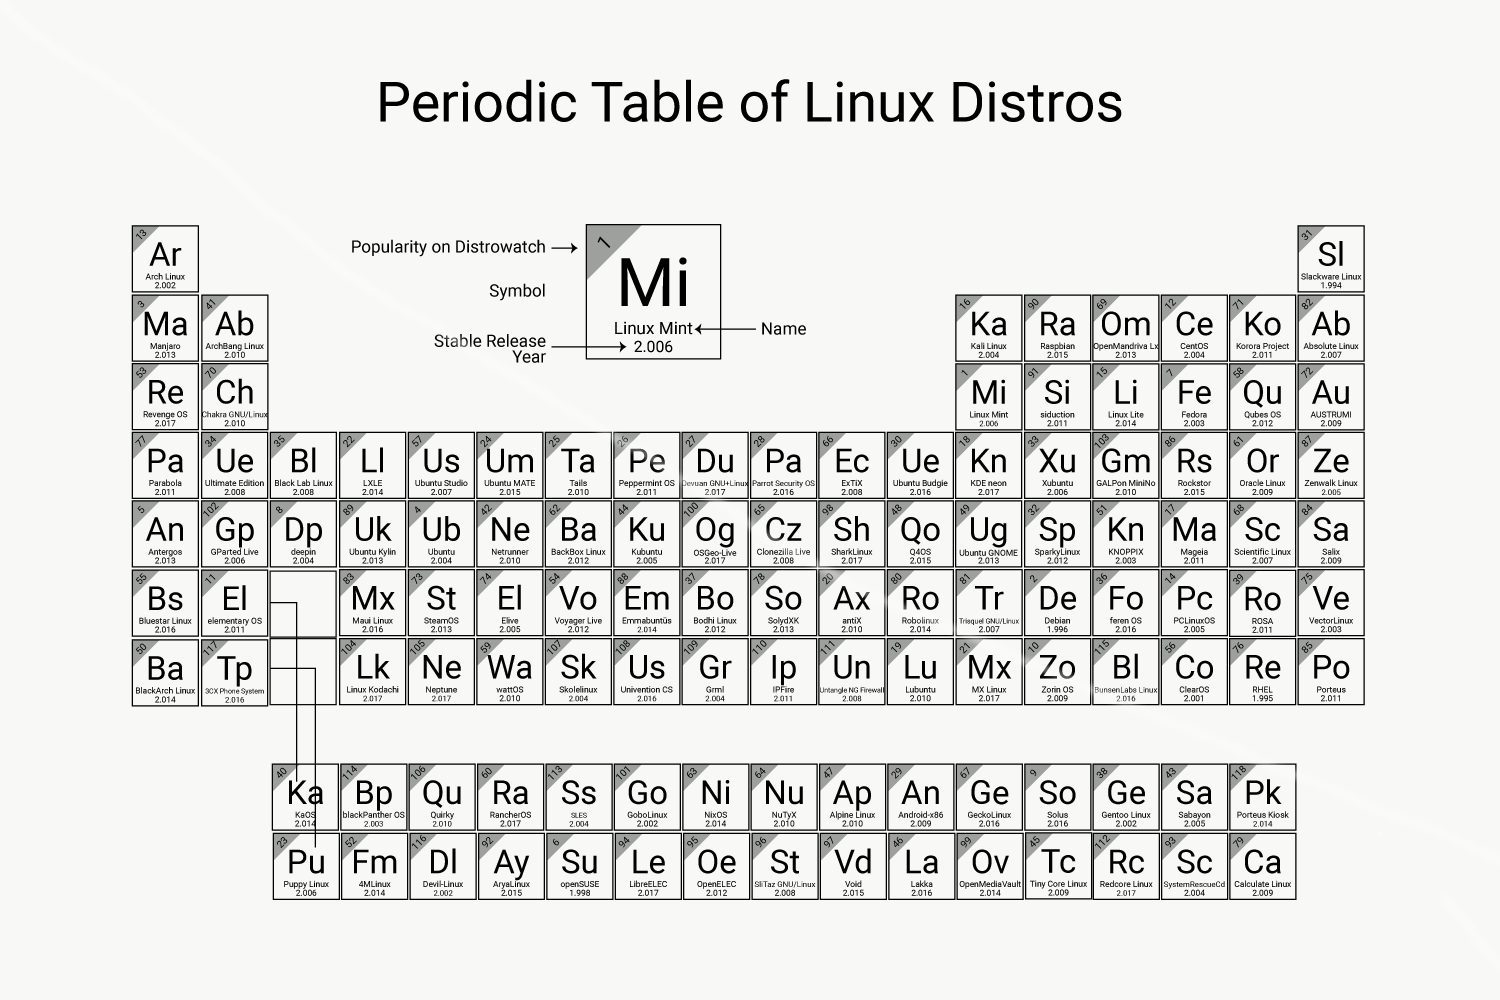
\includegraphics[width=1.0\textwidth,height=0.8\textheight]{periodic-table.png}
\end{frame}

\section{Komunikacija s računalom}
\begin{frame}[t]
\frametitle{Terminal}
\begin{itemize}
  \item ``Uređaj'' koji prima znakove i prikazuje ispis
  \begin{itemize}
    \item Nekada su terminali bili fizički uređaji
    \item Danas su aplikacije koje oponašaju fizičke terminale
  \end{itemize}
  \item Postoji nekoliko emulatora terminala na Unix sustavima
  \begin{itemize}
    \item xterm, rxvt, gnome-terminal, \ldots
  \end{itemize}
  \item Terminali upravljaju unosom i ispisom znakova
  \item Ljuska interpretira značenje znakova
\end{itemize}
\end{frame}

\begin{frame}[t]
\frametitle{Komunikacija sa računalom (1)}
\begin{itemize}
  \item Dva temeljna načina komunikacije
  \begin{itemize}
    \item Kroz grafičko sučelje i putem ljuske/komandne linije
  \end{itemize}
  \item Ljuska je aplikacija(!) koja prihvaća korisnikove naredbe i 
        izvršava ih
  \begin{itemize}
    \item Ljuska olakšava komunikaciju sa sustavom
  \end{itemize}
  \item Ljuska označava spremnost za prihvaćanje naredbi prikazivanjem 
        naredbenog retka (engl. \emph{command prompt})
\end{itemize}
\end{frame}

\begin{frame}[t]
\frametitle{Komunikacija sa računalom (2)}
\begin{itemize}
  \item Kada ljuska pokrene naredbu, čeka da se njeno izvršavanje 
        završi
  \item Za to vrijeme ljuska ne prikazuje narebenu liniju!
  \begin{itemize}
    \item Moguće \textbf{prisilno} zaustaviti naredbu, Ctrl+C
  \end{itemize}
  \item Primjer:
  \begin{itemize}
    \item Pokrenuti naredbu \shell{cat}
  \end{itemize}
\end{itemize}
\end{frame}

\section{Sustav pomoći}
\begin{frame}[t]
\frametitle{Sustav pomoći}
\begin{itemize}
  \item Linux ima sustav pomoći
  \begin{itemize}
    \item Naredba \shell{man}
    \begin{itemize}
      \item Dostupna na svakom Unixu
    \end{itemize}
    \item Naredba \shell{info}
    \begin{itemize}
      \item Dostupna sa GNU alatima
    \end{itemize}
    \item U direktoriju \shell{/usr/share/doc} dosta materijala
  \end{itemize}
  \item Sadrži opise i načine korištenja naredbi, funkcija i 
        konfiguracijskih datoteka
\end{itemize}
\end{frame}

\begin{frame}[t]
\frametitle{Naredba \shell{man} (1)}
\begin{itemize}
  \item Korištenje naredbe man
  \begin{itemize}
    \item Pregled neke upute
    \begin{itemize}
      \item \shell{man <ime naredbe>}
      \item \shell{man <sekcija> <ime naredbe>}
    \end{itemize}
    \item Pretraživanje stranica
    \begin{itemize}
      \item \shell{man -k <ključna riječ>}
      \item \shell{man -f <ime datoteke>}
    \end{itemize}
  \end{itemize}
  \item Primjer: Pregledavanje upute za naredbu \shell{man}
  \begin{itemize}
    \item \shell{man man}
  \end{itemize}
\end{itemize}
\end{frame}

\begin{frame}[t]
\frametitle{Naredba \shell{man} (2)}
\begin{itemize}
  \item Standardni dijelovi \shell{man} stranice
  \begin{itemize}
    \item NAME -- ime i kratki opis
    \item SYNOPSIS -- mogući načini korištenja
    \item DESCRIPTION -- dulji opis što naredba radi
    \item OPTIONS -- opcije koje naredba prihvaća
    \item ENVIRONMENT -- varijable okruženja (o njima kasnije)
    \item AUTHOR -- autor stranice/naredbe
    \item SEE ALSO -- koje su vezane naredbe
  \end{itemize}
\end{itemize}
\end{frame}

\begin{frame}[t]
\frametitle{Naredba \shell{man} (3)}
\begin{itemize}
  \item Opcionalni dijelovi se stavljaju unutar $[$ i $]$
  \item Ponavljanje se označava sa \ldots
  \item Izlazak iz pregledavanja upute
  \begin{itemize}
    \item malo slovo \shell{q}
  \end{itemize}
\end{itemize}
\end{frame}

\section{Prikaz sadržaja direktorija}
\begin{frame}[t]
\frametitle{Prikaz sadržaja direktorija}
\begin{itemize}
  \item Naredba \texttt {ls} (engl. \emph{list})
  \begin{itemize}
    \item Prva akcija nakon pokretanja ljuske na nepoznatom sustavu
    \item bez parametara: popis svih datoteka i direktorija, poredan
          abecednim redom, odozgo prema dolje te s lijeva na desno
  \end{itemize}
  \item \textbf {Linux razlikuje velika i mala slova}
\end{itemize}
\end{frame}

\section{Naredbe}
\begin{frame}[t]
\frametitle{Naredbe (1)}
\begin{itemize}
  \item Naredbe se pokreću na sljedeći način
  \begin{itemize}
    \item[] \textless naredba\textgreater \textless opcije\textgreater 
          \textless arugmenti\textgreater
  \end{itemize}
  \item Argumenti označavaju nad čime se vrši naredba
  \begin{itemize}
    \item Često datoteke
    \item Ponekad nisu potrebni
    \begin{itemize}
      \item Primjer \texttt{ls}
    \end{itemize}
    \item Sve piše u man stranicama
  \end{itemize}
\end{itemize}
\end{frame}

\begin{frame}[t]
\frametitle{Naredbe (2)}
\begin{itemize}
  \item Opcije utječu na ponašanje naredbe
  \begin{itemize}
    \item duge opcije (engl. \emph{long options}) počinju s ``-{}-''  
    \item kratke opcije (engl. \emph{short options}) počinju s ``-''
  \end{itemize}
  \item Naredbe obično imaju različite opcije za isto ponašanje
  \begin{itemize}
    \item Primjer: \texttt{man -k regex} \textbf{ili}
          \texttt{man --apropos regex}
  \end{itemize}
  \item Duge opcije su često opisne zbog lakšeg razumijevanja
\end{itemize}
\end{frame}

%\section{Naredba \texttt{ls}}
\begin{frame}[t]
\frametitle{Naredba \texttt{ls} (1)}
\begin{itemize}
  \item Naredba \texttt{ls} prihvaća niz opcija
  \item Često korištena opcije je \texttt{-l} (engl. \emph{long})
  \begin{itemize}
    \item Ispisuje detalje o datotekama i direktorijima
  \end{itemize}
  \item Primjer: Izvršiti sljedeću naredbu
  \item[] \small\texttt{\$ ls -l /bin/sh}
  \item[] \small\texttt{lrwxrwxrwx 1 root root 4 2010-04-29 10:44 /bin/sh 
                        -> bash}
\end{itemize}
\end{frame}

\begin{frame}[t]
\frametitle{Naredba \texttt{ls} (2)}
\begin{itemize}
  \item Stupci kod korištenja \texttt{ls} naredbe s \texttt{-l} opcijom
  \begin{itemize}
    \item Tip datoteke, dozvole, broj referenci, vlasnik, grupa, veličina
          u oktetima, vrijeme zadnje promijene, ime datoteke
  \end{itemize}
  \item Često \texttt{ls} implicitno dodaje opciju \texttt{-{}-color}
\end{itemize}
\end{frame}

\begin{frame}[t]
\frametitle{Naredba \texttt{ls} (3)}
\begin{itemize}
  \item Naredbi \texttt{ls} moguće je zadati i ime datoteke/direktorija
  \begin{itemize}
    \item niz odvojen prazninama (označen s \ldots u \texttt{man})
  \end{itemize}
  \item Primjer
  \item[] \small\texttt{\$ ls -l /bin/sh}
  \item[] \small\texttt{lrwxrwxrwx 1 root root 4 2010-04-29 10:44 /bin/sh 
                        -> bash}
  \item Opcija \texttt{-h} (engl. \emph{human readable})
  \begin{itemize}
    \item U kombinaciji s \texttt{-l} ispisuje veličine u čitljivijem
          formatu
  \end{itemize}
\end{itemize}
\end{frame}

\section{Skrivene datoteke}
\begin{frame}[t]
\frametitle{Skrivene datoteke}
\begin{itemize}
  \item Skrivene datoteke su skrivene u svrhu ljepšeg/jednostavnijeg ispisa, te kako se ne bi slučajno oštetile nepažnjom korisnika
  \item Na Unix/Linux operacijskom sustavu datoteke čija imena započinju
        točkom su \textbf{skrivene datoteke}
  \begin{itemize}
    \item Ne ispisuju se prilikom izvršavanja naredbe \texttt{ls}, osim
          ako to ne zatražimo
  \end{itemize}
\end{itemize}
\end{frame}

\section{Direktoriji}
\begin{frame}[t]
\frametitle{Direktoriji}
\begin{itemize}
  \item Direktoriji su organizirani kao stablo
  \item U Unix operacijskom sustavu nema diskova
  \begin{itemize}
    \item Sve je \textbf{jedno} stablo direktorija s \textbf{jednim} 
          korijenom
  \end{itemize}
  \centering
  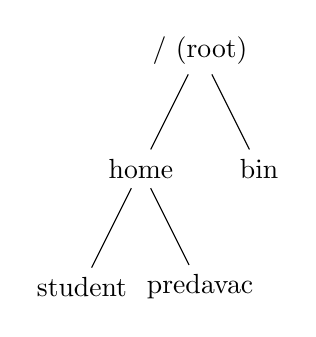
\begin{tikzpicture}
    \node {/ (root)}
        child { 
          node {home} 
          child {node {student} }
          child {node {predavac} }
        }
        child { node {bin} }
    ;
\end{tikzpicture}
\end{itemize}
\end{frame} 


\begin{frame}[t]
\frametitle{Trenutni direktorij}
\begin{itemize}
  \item Trenutni (tekući, radni) direktorij je direktorij u kojem se
        nalazimo
  \begin{itemize}
    \item Korisnik ili aplikacija
  \end{itemize}
  \item Možemo saznati koji je radni direktorij naredbom \texttt{pwd} 
        \\(engl. \emph{print working directory})
\end{itemize}
\end{frame}

\begin{frame}[t]
\frametitle{Matični direktorij}
\begin{itemize}
  \item Svaki korisnik ima matični (engl. \emph{home}) direktoriji
  \begin{itemize}
    \item Služi za spremanje osobnih podataka i postavki
    \item Korisnik ima ovlasti za pisanje i brisanje unutar svog matičnog
          direktorija
    \item Izvan matičnog direktorija \textbf{nije dozvoljeno} pisanje 
          korisnicima koji nisu administratori
  \end{itemize}
  \item Neposredno nakon pokretanja ljuske, trenutni direktorij je matični
        direktorij 
\end{itemize}
\end{frame}

\begin{frame}[t]
\frametitle{Relativna i apsolutna staza (1)}
\begin{itemize}
  \item Položaj datoteke ili direktorija na Unix/Linux sustavu može se 
        zadati
  \begin{itemize}
    \item Apsolutno - počinje znakom ``\texttt{/}''
    \begin{itemize}
      \item[] Primjer: \texttt{/home/student/okosl}
    \end{itemize}
    \item Relativno 
    \begin{itemize}
      \item[] Primjer: \texttt{student/okosl}
    \end{itemize}
  \end{itemize}

  \item Relativna staza ovisi o trenutnom direktoriju
  \begin{itemize}
    \item Može se zadati samo za direktorije koji su niže u hijerarhiji
    \item Ako ste u direktoriju \shell{/home}, apsolutna staza za
          \textbf{student/okosl} je \textbf{/home/student/okosl}
  \end{itemize}
\end{itemize}
\end{frame}

\begin{frame}[t]
\frametitle{Relativna i apsolutna staza(2)}
\begin{itemize}
  \item Znak ``\texttt{/}'' označava korijenski direktorij
  \begin{itemize}
    \item Kod staze znači da je sljedeći direktorij poddirektorij
          prethodnog
  \end{itemize}
  \centering
  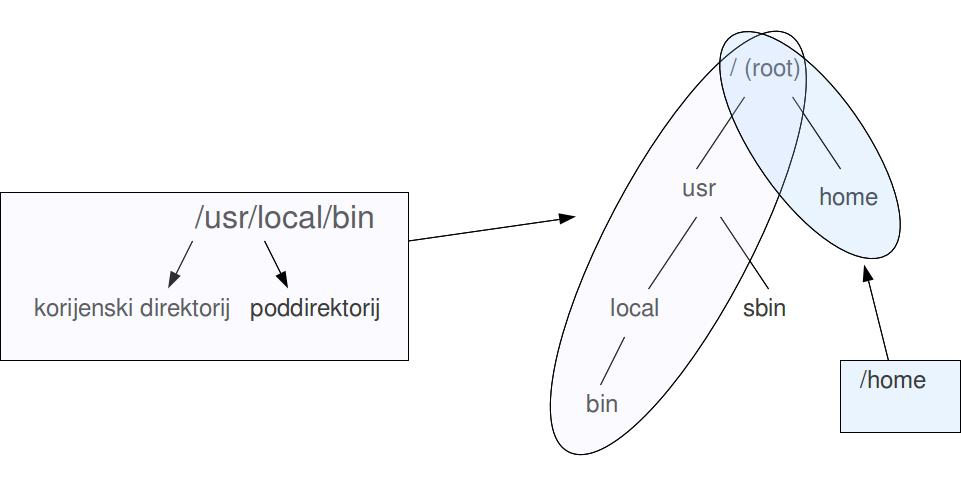
\includegraphics[scale=0.3]{filetree-detail.jpg}
\end{itemize}
\end{frame}

\begin{frame}[t]
\frametitle{Stvaranje direktorija}
\begin{itemize}
  \item Stvaranje novog direktorija obavlja se naredbom \texttt{mkdir}
  \begin{itemize}
    \item Argument je relativno ili apsolutno ime direktorija koji se
          stvara
  \end{itemize}
  \item Naredba \texttt{mkdir} prihvaća opciju \texttt{-p}
  \begin{itemize}
    \item Stvara sve potrebne poddirektorije ako ne postoje
  \end{itemize}
\end{itemize}
\end{frame} 

\begin{frame}[t]
\frametitle{Prikaz sadržaja direktorija}
\begin{itemize}
  \item Naredba \texttt{ls} ispisuje sadržaj direktorija
  \item Opcijom \texttt{-d} ne izlistava se sadržaj direktorija već 
        informacije o samom direktoriju
\end{itemize}
\end{frame}
    

\begin{frame}[t]
\frametitle{Promjena direktorija (1)}
\begin{itemize}
  \item Promjena direktorija obavlja se naredbom \texttt{cd} (engl. 
        \emph{change directory})
  \item Novi direktorij se zadaje 
  \begin{itemize}
    \item relativno u odnosu na tekući direktorij
    \item apsolutno u odnosu na korijenski direktorij  
  \end{itemize}
  \item Naredba \texttt{cd} bez argumenata vraća u matični direktorij
\end{itemize}
\end{frame}

\begin{frame}[t]
\frametitle{Posebni direktoriji (1)}
\begin{itemize}
  \item Svaki direktorij sadrži dva posebna direktorija
  \begin{itemize}
    \item \texttt{..} roditeljski direktorij (engl. \emph{parent directory})
    \item \texttt{.} tekući direktorij (engl. \emph{current directory})
  \end{itemize}
  \item Primjeri
  \begin{itemize}
    \item \texttt{cd . } 
    \begin{itemize}
      \item Mijenja direktorij u tekući direktorij, efektivno nema 
               promjene
    \end{itemize}
    \item \texttt{cd .. }
    \begin{itemize}
      \item Mijenja trenutni direktorij u direktorij iznad
    \end{itemize}
  \end{itemize}
\end{itemize}
\end{frame}

\begin{frame}[t]
\frametitle{Posebni direktoriji (2)}
\begin{itemize}
  \item Koriste se za relativno \emph{adresiranje} direktorija
  \item Ne mogu ići van korijenskog direktorija, tj.
  \begin{itemize}
    \item[] \texttt{/../../} je isto što i \texttt{/}
  \end{itemize}
  \item Česta pogreška korisnika DOS-a
  \begin{itemize}
    \item Upisivanje \texttt{cd..} (bez razmaka)
    \item Na Unixu to je posebna naredba (\emph{.} može biti sastavni dio 
          imena)
  \end{itemize}
\end{itemize}
\end{frame}

\begin{frame}[t]
\frametitle{Posebni direktoriji (3)}
\begin{itemize}
  \item Posebni direktoriji se mogu koristiti u imenima datoteka
  \flushleft
  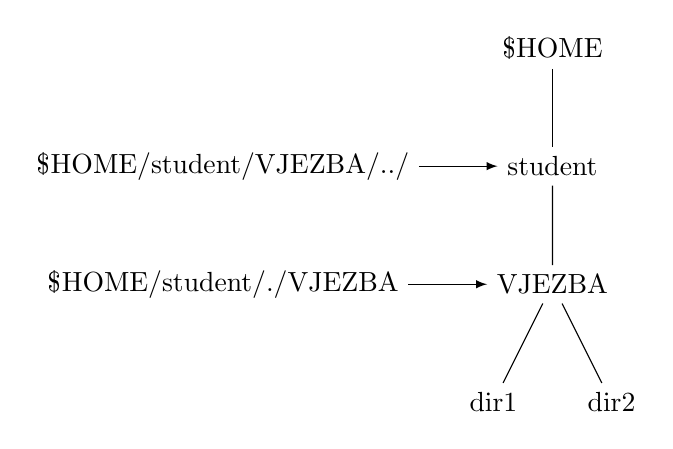
\begin{tikzpicture}[auto, >=latex]
  \node{\$HOME}
    child {
      node (a) {student} 
      child {
        node (b) {VJEZBA}
        child { node {dir1} }
        child { node {dir2} }
      }
    }
  ;
  \node (c) [left=1cm of a] {\$HOME/student/VJEZBA/../}; 
  \node (d) [left=1cm of b] {\$HOME/student/./VJEZBA};
  \draw[->] (c) -- (a);
  \draw[->] (d) -- (b);
  \end{tikzpicture}
\end{itemize}
\end{frame}

\section{Skripte u bashu}
\begin{frame}[t]
\frametitle{Skripte}
\begin{itemize}
  \item Skripta je niz naredbi zapisan u tekstualnu datoteku, a za čije izvršavanje nije potreban compiler
  \item Inače bi korisnik morao unostit svaku naredbu zasebno u ljusku
  \item Kratica za skriptu je .sh, te se pokreće naredbom \shell{bash <ime\_skripte>}
\end{itemize}
\end{frame}

\begin{frame}[t]
\frametitle{Primjer skripte}
\begin{itemize}
  \item \#!/bin/bash \\ mkdir radno \\ echo pozdrav\_ekipa \\ ls -lh
\end{itemize}
\end{frame}

\section{Pregled naredbi}
\begin{frame}[t]
\frametitle{Pregled naredbi}
\begin{tabular}{| l | c |} \hline
  \shell{man <ime naredbe>} & opis određene naredbe \\ \hline
  \shell{ls} & popis svih datoteka i direktorija \\ \hline
  \shell{pwd} & trenutni (radni) direktorij \\ \hline
  \shell {mkdir} & stvaranje novog direktorija \\ \hline
  \shell{cd} & promjena trenutnog direktorija \\ \hline
  \shell{bash <ime skripte>} & pokretanje skripte \\ \hline

\end{tabular}
\end{frame}

\begin{frame}[t]
\frametitle{Upravljanje paketima}
\begin{itemize}
  \item paket je program
  \item \texttt{yum, apt, pacman, zypper \ldots}
  \item \texttt{software manager}
  \item repozitoriji
  \item \texttt{apt-get update}
  \item \texttt{apt-get install git}
\end{itemize}
\end{frame}

\begin{frame}[t]
\frametitle{Literatura}
\begin{itemize}
  \item \url{http://www.troubleshooters.com/linux/info.htm}
  \item \url{http://www.schweikhardt.net/man_page_howto.html\#q3}
  \item \url{http://www.debian.org/doc/debian-policy/ch-docs.html}
  \item \url{http://www.unix.org/what_is_unix/history_timeline.html}
  \item \url{http://distrowatch.com/dwres.php?resource=major}
\end{itemize}
\end{frame}


\end{document}
